\documentclass[a4paper,12pt]{article}
\usepackage{mathtools,amsfonts,amssymb,amsmath, bm,commath,multicol}
\usepackage{algorithmicx, tkz-graph, algorithm, fancyhdr, pgfplots}
\usepackage{fancyvrb}

\usepackage[noend]{algpseudocode}


\pagestyle{fancy}
\fancyhf{}
\rhead{21/2/2017 ::: Group yadadya}
\lhead{Pricing Financial Derivative ::: Problemset 2}
\rfoot{\thepage}


\DefineVerbatimEnvironment{juliaout}{Verbatim}{}
\DefineVerbatimEnvironment{juliacode}{Verbatim}{fontshape=sl, fontsize=\tiny}
\DefineVerbatimEnvironment{juliaterm}{Verbatim}{}


\begin{document}

\section{}

\subsection*{Solution}

Tha solution:
%
\begin{align*}
S_t &= e^{\sigma W_t + (\mu - \frac{\sigma^2}{2})t} \\
S_t &= e^{\frac{3}{2}W_t + \frac{7}{8}t}
\end{align*}

\subsection*{Code}
\begin{juliacode}
using Distributions
using Gadfly

function make_walk(steps::AbstractArray{Float64,1}, start = 0.0)
    reduce((a,b) -> append!(a, a[end] + b), [start], steps)
end

make_time(N, T) = range(0, T/N, N)
brownian(N, T, start = 0.0) = make_walk(rand(Normal(0, sqrt(T/N)), N-1), start)

# Helper to cover the normal distributions from a brownian motion
get_steps(B) = [B[i] - B[i-1] for i in 2:length(B)]

geom(w, mu, sigma, t) = exp(sigma*w + (mu - sigma^2/2)*t)
geometric(brownian, time, mu, sigma) = [geom(b,mu,sigma,t) for (b,t) in zip(brownian, time)]

function eulers_method(B, N, T, mu, sigma, start = 1.0)
    d = T/N
    norms = get_steps(B)
    eul(x,n) = x + sigma*x*n + mu*x*d
    reduce((a,b) -> append!(a, eul(a[end], b)), [start], norms)
end

function plot_em(N, T, mu = 2, sigma = 1.5, start = 1.0)
    # Basix
    time = make_time(N, T)
    B = brownian(N, T)
    # Our two lines
    path = geometric(B, time, mu, sigma)
    euler = eulers_method(B, N, T, mu, sigma, start)
    # Plotem
    plot(layer(x = time, y = path, Geom.line,
               Theme(default_color=colorant"rgba(220,130,50,0.75)")),   
         layer(x = time, y = euler, Geom.line),
         Theme(default_color=colorant"rgba(130,230,50,0.75)"))
end
\end{juliacode}



\subsection*{Plot for N = 100, T = 1}
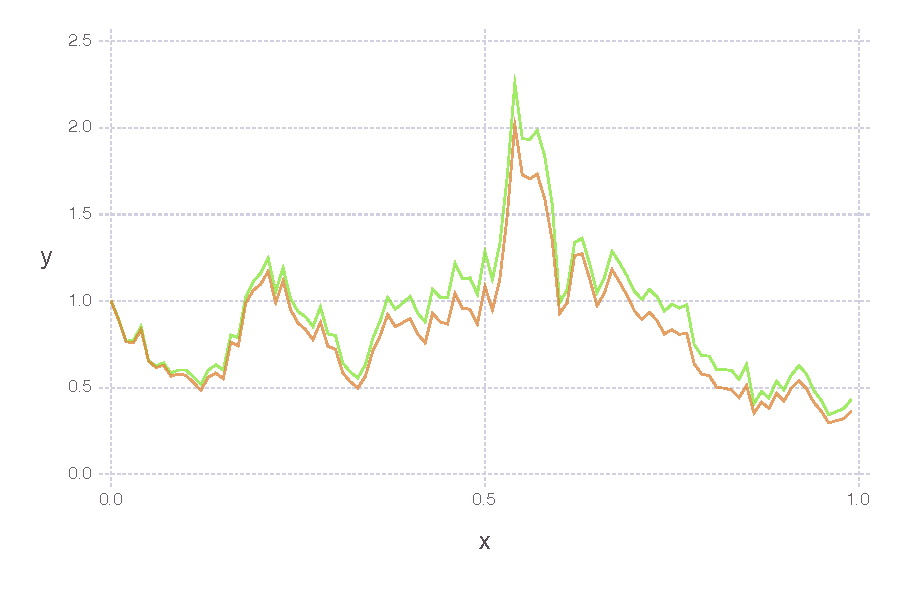
\includegraphics[width=\linewidth]{figures/problemset_2_1.pdf}



\subsection*{Plot for N = 250, T = 1}
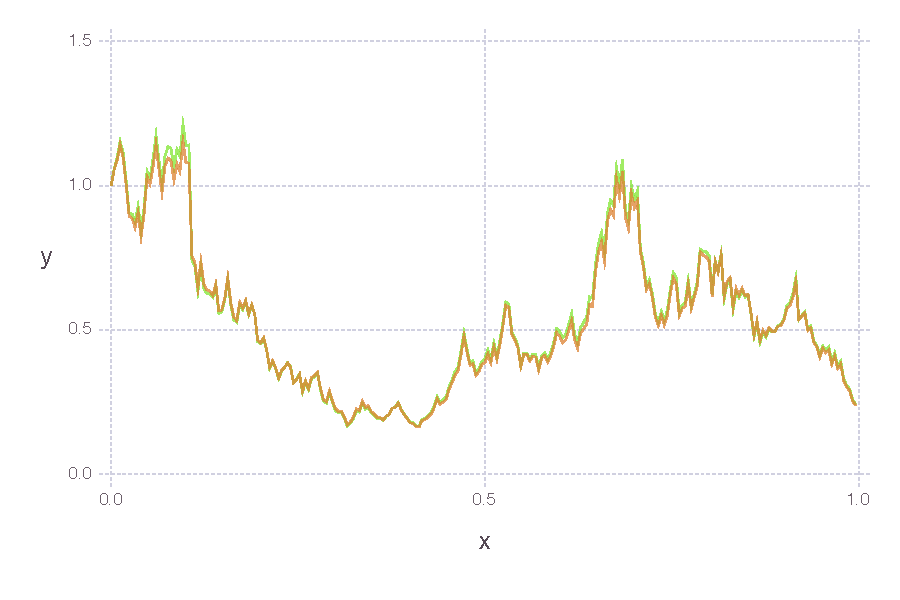
\includegraphics[width=\linewidth]{figures/problemset_3_1.pdf}



\subsection*{Plot for N = 1000, T = 1}
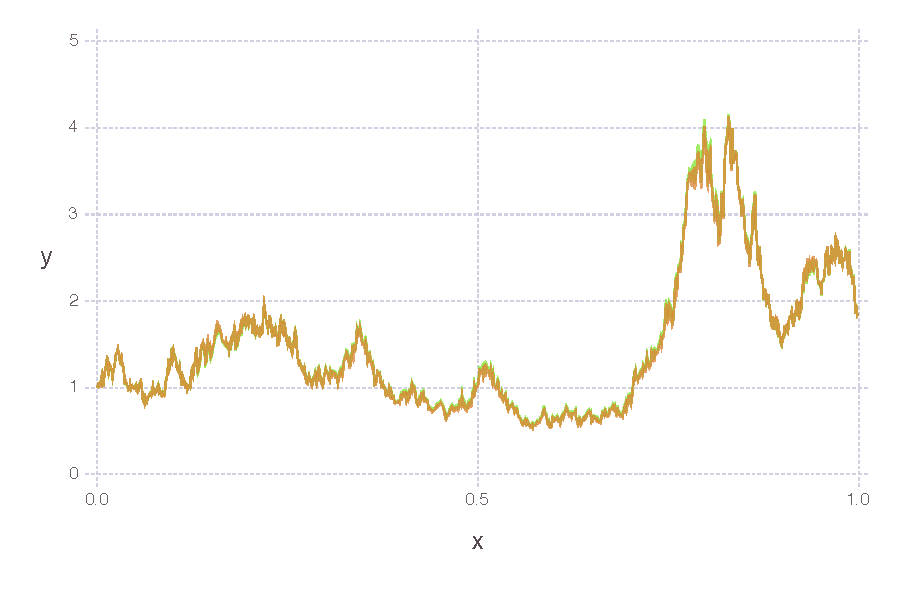
\includegraphics[width=\linewidth]{figures/problemset_4_1.pdf}



\end{document}